\documentclass[a4paper]{article}

\title{Lecture 2: Seqences, Limits and Infinites}
\author{Shashank Vatedka}

\usepackage{basicreq}
\usepackage{./teaching_doc_macros}
\DeclareMathOperator*{\maxi}{Max}
%\DeclareMathOperator*{\lim}{Lim}
\begin{document}

%FILL IN THE RIGHT INFO.
%\lecture{**LECTURE-NUMBER**}{**UNIT**}{**LECTURER**}{**SCRIBE**}
\lecture{2}{SEQUENCES, LIMITS AND INFINITES}{Shashank Vatedka}{EE20RESCH14005}
%\footnotetext{These notes are partially based on those of Nigel Mansell.}

% **** YOUR NOTES GO HERE:
\section{GIST OF LECTURE 1}
In the last lecture, we have seen the introduction topics such as\\
\begin{enumerate}
\item	What does a general communication system look like?
\begin{figure}[!ht]
\centering
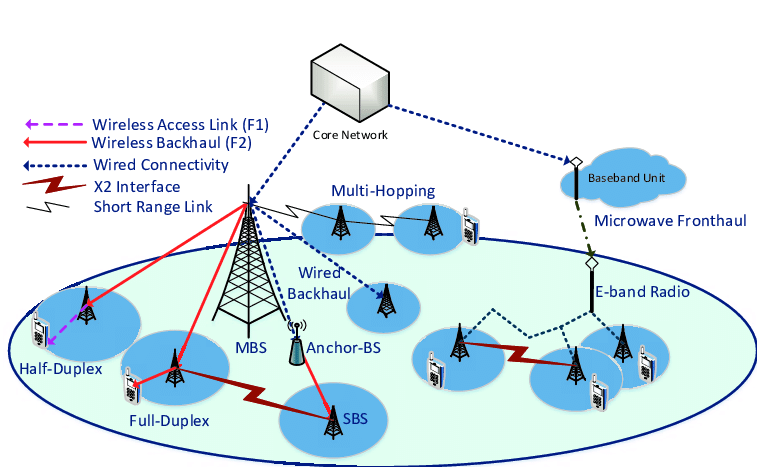
\includegraphics[width=6.0cm]{wireless image 1.png}
\caption{General Communication Systems}\label{fig:1}
\end{figure} \\
A general communication system consists of user equipments(source nodes) connected to base stations through a wireless links otherwise called channels which are noisy. These Base Stations are inturn connected to a back haul network which connects to a core network via a wired/ optical link. They are to support a large number of users.\\
\\
In such systems, primary goal will be designing a noise free communciation system which require modelling of source as well as channel. 
\\
\item \textbf{Single User/ Point-to-Point System}.\\
\begin{figure}[!ht]
\centering
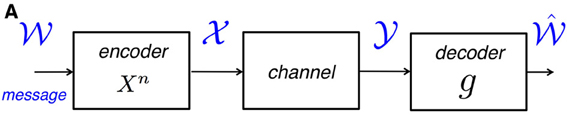
\includegraphics[width=6.0cm]{simple_encoder_decoder.png}
\caption{Single User/ Point-to-Point System}\label{fig:2}
\end{figure} \\
In a point-to-point/ single user communication system which is shown in above figure, the max rate at which the communication may take place is given by
\begin{align}
\begin{split}
	\Rightarrow R = \frac{k}{n}
\end{split}
\end{align}
where k is number of useful message bits taken by encoder and generate codewords of n bits length.It may appear very simple. To measure the performance of the system, Rate(code rate) and $P_e$(bit error rate) are used. The channel is defined by the transition probability matrix i.e. $P_\frac{Y}{X}$. The capacity of the channel is given by\\
\\
\begin{align}
\begin{split}
C=\maxi_{\mathbf{P_X}} I(X;Y)\\
\end{split}
\end{align}
\\
From Shannon Channel Coding Theorem, the design considerations can be put up together as follows:
\\
\\
\begin{align}
\begin{split}
\lim_{n \to \infty} R \approx I(X;Y)\\
\lim_{n \to \infty} P_e \approx 0\\
\end{split}
\end{align}
\\
\item \textbf{Multi-User Systems}.\\
\begin{figure}[!ht]
\centering
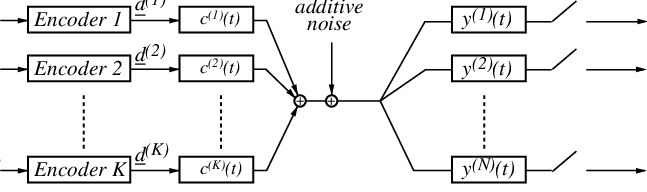
\includegraphics[width=6.0cm]{multi-user-systems.png}
\caption{Multi-User System}\label{fig:3}
\end{figure} \\
\\
In Multi-User Systems, goal is to receive the distinct number of messages without any loss or interference within the power constraints. The rate of transmission are given as below.
\\
\\
\begin{align}
\begin{split}
	\Rightarrow R_1 = \frac{k_1}{n}\\
	\Rightarrow R_2 = \frac{k_2}{n}...\\
\end{split}
\end{align}
\begin{enumerate}
\item How to mitigate effects of Interference?\\
By using a type of scheduling mechanism, one can avoid the interference caused by multiple signals generated by multiple users such as TDMA(most commonly used), FDMA etc.,.
\\
\item How to measure performance?\\
Consider only 2 users are trying to communicate using a system. Here assume the noise is gaussian i.e. $W_i \sim \mathcal{N}(\mu = 0,\,\sigma^{2})$
In an AWGN channel, the max rate  is  given by
\begin{align}
\begin{split}
R_{max} = C = \frac{1}{2}*log_2(1+\frac{P}{\sigma^2})\\
where \frac{P}{\sigma^2} = SNR.
\end{split}
\end{align}
\\
When any scheduling is done, the max rate is dependent on the time allotted or divided between the users. The max rates as per the user is given as below:
\begin{align}
\begin{split}
	\Rightarrow R_1 \leq \alpha C\\
	\Rightarrow R_2 \leq (1-\alpha C)\\
	where C = \frac{1}{2}*log_2(1+\frac{P}{\sigma^2})\\
\end{split}
\end{align}
If the plot of above rates is carried out, it will look below:
\begin{figure}[!ht]
\centering
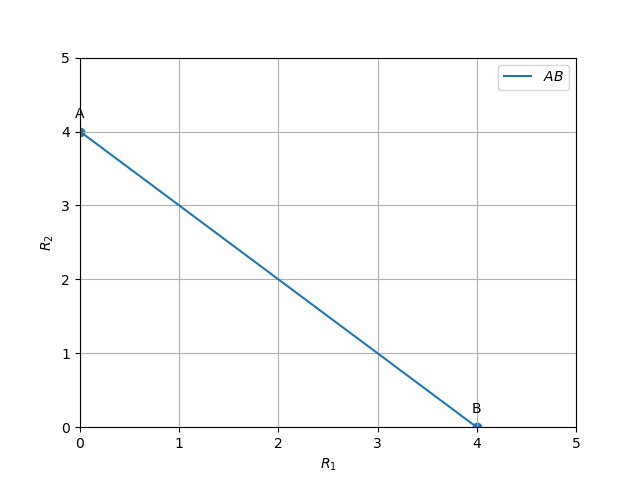
\includegraphics[width=6.0cm]{R1_R2.png}
\caption{Rate Performance Graph}\label{fig:4}
\end{figure} \\
\end{enumerate}
\item This performance is obtained by simply following simple TDMA techniques. Can we do better?
\\
The answer is Yes. The rate performance in a multi-user system can be improved by using a procedure called Successive Interference Cancellation(\textbf{SIC}). In this interference caused by another user is treated as noise and the rate of user 1 is calculated. Once the rate of user 1 is calculated, then the user 2 rate is calculated. The rates can be obtained as below:\\
\\
\\
\\

\begin{align}
\begin{split}
	\Rightarrow R_1 = C = \frac{1}{2}*log_2(1+\frac{P}{P+\sigma^2})\\
	\Rightarrow R_2 = \frac{1}{2}*log_2(1+\frac{P}{\sigma^2})\\
\end{split}
\end{align}
\\
\\
\\

The plot of $R_1$ vs $R_2$ is shown below:
\begin{figure}[!ht]
\centering
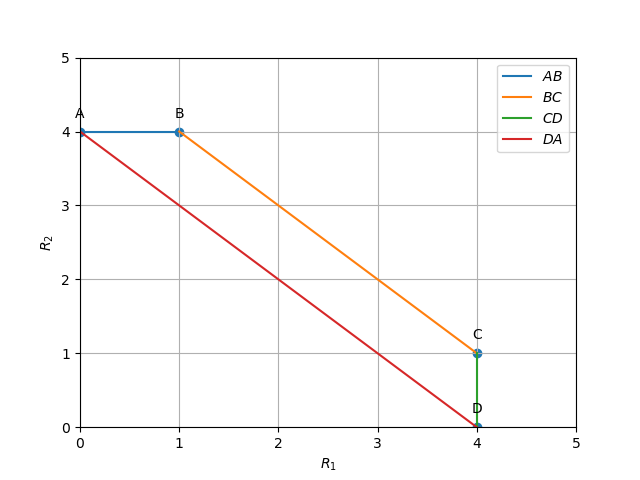
\includegraphics[width=6.0cm]{R1_R2_better.png}
\caption{Rate Performance Graph through SIC}\label{fig:5}
\end{figure} \\
\\There are more techniques which will further enhance of multi-user systems which will be studied in this course.
\end{enumerate}
\bigskip
\section{Commonly used Notions}
\begin{enumerate}
\item \textbf{R} - Rate
\item $P_e$ - Probability of Error
\item X, Y, Z...  - Random Varaibles
\item x,y,z..... - Deterministic Variables
\item $\bR$ - Real Numbers, $\bZ$ - Integers, $\bN$ - Natural numbers
\item Pr[X=x] - Probability Distributive Function (PDF)
\item $P_x$ - Probability Mass Function (pmf)
\item $f_x$ - Probability Density Function (pdf)
\item $P_{\frac{x}{y}}(\frac{X}{Y})$ - Conditional pmf
\item $f_{\frac{x}{y}}(\frac{X}{Y})$ - Conditional pdf
\end{enumerate}

% Some general latex examples and examples making use of the
% macros follow.  
%**** IN GENERAL, BE BRIEF. LONG SCRIBE NOTES, NO MATTER HOW WELL WRITTEN,
%**** ARE NEVER READ BY ANYBODY.






\end{document}

